%%%%%%%%%%%%%%%%%%%%%%%%%%%%%%%%%%%%%%%%%
% Jacobs Landscape Poster
% LaTeX Template
% Version 1.1 (14/06/14)
%
% Created by:
% Computational Physics and Biophysics Group, Jacobs University
% https://teamwork.jacobs-university.de:8443/confluence/display/CoPandBiG/LaTeX+Poster
% 
% Further modified by:
% Nathaniel Johnston (nathaniel@njohnston.ca)
%
% This template has been downloaded from:
% http://www.LaTeXTemplates.com
%
% License:
% CC BY-NC-SA 3.0 (http://creativecommons.org/licenses/by-nc-sa/3.0/)
%
%%%%%%%%%%%%%%%%%%%%%%%%%%%%%%%%%%%%%%%%%

%----------------------------------------------------------------------------------------
%	PACKAGES AND OTHER DOCUMENT CONFIGURATIONS
%----------------------------------------------------------------------------------------

\documentclass[final]{beamer}

\usepackage[scale=1.24]{beamerposter} % Use the beamerposter package for laying out the poster
\usepackage{multirow}
\usepackage{array,booktabs}
\newcolumntype{M}[1]{>{\centering\arraybackslash}m{#1}}

\usetheme{confposter} % Use the confposter theme supplied with this template

\setbeamercolor{block title}{fg=ngreen,bg=white} % Colors of the block titles
\setbeamercolor{block body}{fg=black,bg=white} % Colors of the body of blocks
\setbeamercolor{block alerted title}{fg=white,bg=dblue!70} % Colors of the highlighted block titles
\setbeamercolor{block alerted body}{fg=black,bg=dblue!10} % Colors of the body of highlighted blocks
% Many more colors are available for use in beamerthemeconfposter.sty

%-----------------------------------------------------------
% Define the column widths and overall poster size
% To set effective sepwid, onecolwid and twocolwid values, first choose how many columns you want and how much separation you want between columns
% In this template, the separation width chosen is 0.024 of the paper width and a 4-column layout
% onecolwid should therefore be (1-(# of columns+1)*sepwid)/# of columns e.g. (1-(4+1)*0.024)/4 = 0.22
% Set twocolwid to be (2*onecolwid)+sepwid = 0.464
% Set threecolwid to be (3*onecolwid)+2*sepwid = 0.708

\newlength{\sepwid}
\newlength{\onecolwid}
\newlength{\twocolwid}
\newlength{\threecolwid}
\setlength{\paperwidth}{48in} % A0 width: 46.8in
\setlength{\paperheight}{36in} % A0 height: 33.1in
\setlength{\sepwid}{0.024\paperwidth} % Separation width (white space) between columns
\setlength{\onecolwid}{0.301\paperwidth} % Width of one column
\setlength{\twocolwid}{0.627\paperwidth} % Width of two columns
\setlength{\threecolwid}{0.951\paperwidth} % Width of three columns
\setlength{\topmargin}{-0.00000005in} % Reduce the top margin size
%-----------------------------------------------------------

\usepackage{graphicx}  % Required for including images

\usepackage{booktabs} % Top and bottom rules for tables
\renewcommand{\arraystretch}{1.2} 

%----------------------------------------------------------------------------------------
%	TITLE SECTION 
%----------------------------------------------------------------------------------------

\title{Who's to say what's funny? \\ A computer using Language Models and Deep Learning, That's Who!} % Poster title

\author{\textbf{Xinru Yan \& Ted Pedersen} \\ 
\vspace{4mm}
\normalsize \href{mailto:\{yanxx418,tpederse\}@d.umn.edu}{\{yanxx418,tpederse\}@d.umn.edu}}
% Author(s)

\institute{Department of Computer Science University of Minnesota Duluth} % Institution(s)


%----------------------------------------------------------------------------------------

\begin{document}

\addtobeamertemplate{block end}{}{\vspace*{2ex}} % White space under blocks
\addtobeamertemplate{block alerted end}{}{\vspace*{2ex}} % White space under highlighted (alert) blocks

\setlength{\belowcaptionskip}{1ex} % White space under figures
\setlength\belowdisplayshortskip{3ex} % White space under equations

\begin{frame}[t] % The whole poster is enclosed in one beamer frame

\begin{columns}[t] % The whole poster consists of three major columns, the second of which is split into two columns twice - the [t] option aligns each column's content to the top

\begin{column}{\sepwid}\end{column} % Empty spacer column

\begin{column}{\onecolwid} % The first column

%----------------------------------------------------------------------------------------
%	INTRODUCTION
%----------------------------------------------------------------------------------------

\begin{block}{The Problem}
\begin{itemize}
%\textit{Humor} is a defining characteristic of human beings. 
%\textit{Computational humor} ties together ideas from psychology, linguistics, and cognitive science. 
\item \large Traditional humor detection: \textit{binary classification} \\
\large \textbf{Our focus}: learn a \textit{continuous} and \textit{subjective} sense of humor 
from tweets submitted to the \textit{@midnight} show in response to hashtags 
by using \textbf{Ngram Language Models} (LMs) and \textbf{Deep Learning} (DL) methods 

\item We participated in \textbf{SemEval-2017 Task 6} 
\#HashtagWars: Learning a Sense of Humor ~\cite{PotashRR17}:

\begin{itemize} 
\item \large Tweets are in three baskets: top most funny tweet, next nine most funny tweets and all remaining
\vspace{4mm}
\item \large \textbf{Two Subtasks} 
\begin{itemize}
\item \large A: Pairwise Comparison -- a system should choose a funnier of two tweets given a hashtag file
\item \large B: Semi-Ranking -- a system should categorize tweets into the right baskets given a hashtag file
\end{itemize}
\vspace{4mm}
\item \textbf{Dataset}
\begin{itemize}
\item \large \textit{Tweet Data}: provided by the task, 106 hashtag files, about 21,580 tokens
\item \large \textit{News Data}: We used 6.2 GB English news, about 2 million tokens \cite{EMNLP}
\end{itemize}
\end{itemize}
\end{itemize}
\end{block}

\begin{alertblock}{\small{Examples from \#BreakUpIn5Words (Trigram LM, News Data)}}

\begin{table}[h!]
\centering
\begin{tabular} {  l | l | l | c }
\toprule
\multicolumn{1}{c|}{Tweet} & \textit{@midnight} & LM & DL\\
\hline
It's not you, it's meth. & funniest & funny  & \multirow{5}*{\textbf{?}}\\
Hey, can we NOT talk? & funny & funny \\
You need your own Netflix  & funny & not funny \\
Figured I'd try being happy.  & not funny & funny \\
You're a Mac, I'm PC & not funny & not funny \\	
\bottomrule
\end{tabular}
\end{table}
\end{alertblock}
\end{column} % End of the first column

\begin{column}{\sepwid}\end{column} % Empty spacer column

\begin{column}{\onecolwid} % Begin a column which is two columns wide (column 2)

%----------------------------------------------------------------------------------------
%	IMPORTANT RESULT
%----------------------------------------------------------------------------------------



% \begin{columns}[t,totalwidth=\twocolwid] % Split up the two columns wide column

% \begin{column}{\onecolwid}\vspace{-.6in} % The first column within column 2 (column 2.1)

\begin{block}{Language Models}
Ngram LMs learn humor from training data and allow ranking by assigning probability for each statement \cite{Heafield-estimate}\cite{hello}
\begin{figure}
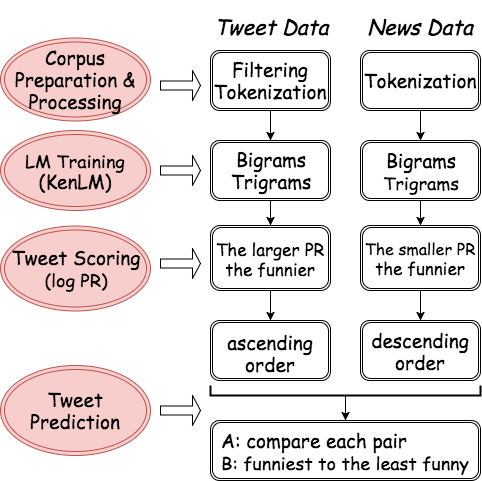
\includegraphics[width=0.77\linewidth]{Method.png} 
\end{figure}
\end{block}

\begin{block}{Language Model Results}
We seek high accuracy for A and low distance for B.
\begin{table}[h!]
\centering
\begin{tabular}{ |p{9cm}|p{9cm}|p{9cm}|p{9cm}|}
\toprule
\multicolumn{1}{|c|}{Dataset} & \multicolumn{1}{|c|} {Ngram} & Accuracy (A) & Distance (B) \\
\hline
\multicolumn{1}{|c|}{\textbf{news}} & \multicolumn{1}{|c|}{\textbf{3}} & \textbf{0.627} (4th) & \textbf{0.872} (1st)\\
\hline
\multicolumn{1}{|c|}{news} & \multicolumn{1}{|c|}{2} & 0.624 & 0.853 \\
\hline
\multicolumn{1}{|c|}{\textbf{tweet}} & \multicolumn{1}{|c|}{\textbf{3}} & \textbf{0.397} (8th) & \textbf{0.967} (8th)\\
\hline
\multicolumn{1}{|c|}{tweet} & \multicolumn{1}{|c|}{2} & 0.406 & 0.944 \\
\bottomrule
\end{tabular}
\end{table}
\begin{itemize}
\item The \textbf{type} and the \textbf{quantity} of the corpora is what really matters --> \textit{more tweet data, less news data}
\item Bigram LMs performed slightly better than trigram LMs 
\\ --> \textit{Unigram} and \textit{character} level LMs 
\end{itemize}
\end{block}
\end{column}

% end of the second column

\begin{column}{\sepwid}\end{column} % Empty spacer column

\begin{column}{\onecolwid} % The third column

\begin{block}{Deep Learning}
\begin{itemize}
\item Humor relies on creative use of language which causes too many OOV 
\begin{itemize}
\item \large Jokes often include puns based on invented words
\\ {\hfil \normalsize Barktender \#DogJobs}
\\ {\hfil \normalsize Tinderella \#UpdateAFairyTale}
\item Token-level LMs can not understand such puns
\item Character-based CNNs (CharCNN) are not dependent on observing tokens in training data
\end{itemize}	
\item Bigram and trigram LMs only use two or three preceding words to predict the next word --> LSTMs are good at making use of sequantial data such as text and are designed for long-term dependencies
\begin{itemize}
\item \large Some hashtags require tweets to have more than three words and some funny tweets are mostly made up of common bigrams or trigrams
\\ {\hfil \normalsize Complaining makes it better \#AmericaIn4Words}
\\ {\hfil \normalsize Romantic dinners with the cats \#BestWeekendIn5Words} 
\end{itemize}
\item Ngram LMs do not include external knowledge such as movie titles and song lyrics --> Create word embeddings from domain specific materials
\item Our plan: use Keras library to train CharCNN + LSTM LMs on both datasets and investigate ways to include domain knowledge word embeddings in the CharCNN + LSTM LM

\end{itemize}

\end{block}

%----------------------------------------------------------------------------------------
%	REFERENCES
%----------------------------------------------------------------------------------------

\begin{block}{References}

\nocite{*} % Insert publications even if they are not cited in the poster
\tiny{\bibliographystyle{unsrt}
\bibliography{sample}\vspace{0.75in}}

\end{block}


% \begin{center}
% \begin{tabular}{c}
% 
\includegraphics[width=0.7\linewidth]{logo.png}\\
% \end{tabular}
% \end{center}

%----------------------------------------------------------------------------------------

\end{column} % End of the third column


\end{columns} % End of all the columns in the poster



\end{frame} % End of the enclosing frame

\end{document}
